% !TeX spellcheck = cs_CZ
\documentclass[a4paper,hidelinks]{report}

\usepackage[utf8]{inputenc}
\usepackage[czech]{babel}
\usepackage{hyperref}
\usepackage{amsmath}
\usepackage{amsfonts}
\usepackage{amssymb}
\usepackage{listingsutf8}
\usepackage[table]{xcolor}
\usepackage{inconsolata}
\usepackage{nameref}
\usepackage{pifont}
\usepackage{placeins}
\usepackage[a4paper,includeheadfoot,margin=3.5cm]{geometry}
\usepackage{multirow}
\usepackage{pdflscape}
\usepackage{graphicx}
\newcommand{\cmark}{\ding{51}}
\newcommand{\xmark}{\ding{55}}

%Vkladani source kodu
\lstdefinestyle{codeInput} { %
	language=C++,
	basicstyle=\ttfamily\footnotesize,
	numberstyle=\scriptsize,
	numbers=left,
	backgroundcolor=\color{gray!10},
	frame=single,
	keepspaces=true,  
	showspaces=false,
	showstringspaces=false,
	showtabs=false,
	tabsize=4,
	rulecolor=\color{black!30},
	escapeinside={\%*}{*)},
	breaklines=true,
	breakatwhitespace=true,
	framextopmargin=2pt,
	framexbottommargin=2pt,
	inputencoding=utf8/latin2,
	extendedchars=true,
	literate=
	{á}{{\'a}}1
	{í}{{\'i}}1
	{é}{{\'e}}1
	{ý}{{\'y}}1
	{ú}{{\'u}}1
	{ó}{{\'o}}1
	{ě}{{\v{e}}}1
	{š}{{\v{s}}}1
	{č}{{\v{c}}}1
	{ř}{{\v{r}}}1
	{ž}{{z}}1
	{ď}{{\v{d}}}1
	{ť}{{\v{t}}}1
	{ň}{{\v{n}}}1                
	{ů}{{\r{u}}}1
	{Á}{{\'A}}1
	{Í}{{\'I}}1
	{É}{{\'E}}1
	{Ý}{{\'Y}}1
	{Ú}{{\'U}}1
	{Ó}{{\'O}}1
	{Ě}{{\v{E}}}1
	{Š}{{\v{S}}}1
	{Č}{{\v{C}}}1
	{Ř}{{\v{R}}}1
	{Ž}{{\v{Z}}}1
	{Ď}{{\v{D}}}1
	{Ť}{{\v{T}}}1
	{Ň}{{\v{N}}}1                
	{Ů}{{\r{U}}}1    	
}
\lstset{style=codeInput}
\renewcommand{\lstlistingname}{Zdrojový kód}
\renewcommand{\lstlistlistingname}{Seznam zdrojových kódů}
\newcommand{\includecode}[3][default]
{\lstinputlisting[caption=#3,label=lst:#1, style=codeInput]{#2}}


\DeclareGraphicsExtensions{.pdf,.png,.jpg}
\usepackage{fancyhdr}
\setlength{\headheight}{15pt}

\pagestyle{fancy}

\fancyhf{}
\fancyfoot[C]{\thepage}
\fancyhead[L]{\textit{ \expandafter\MakeUppercase\expandafter{\leftmark}} }
\fancyhead[R]{\textit{ {\rightmark}} }

\fancypagestyle{plain}{ %
	\fancyhf{} % remove everything
	\fancyfoot[C]{\thepage}
	\renewcommand{\headrulewidth}{0pt} % remove lines as well
	\renewcommand{\footrulewidth}{0pt}
}

\begin{document}
\chapter{Uživatelská dokumentace}
Po zkompilování jsou vytvořeny dvě aplikace - \texttt{Client.exe} a \texttt{Server.exe}. Nejdříve je potřeba spustit server, poté lze pustit klienta. Po jeho spuštění se zobrazí černé okno a konzole kam uživatel zadá IP adresu serveru("127.0.0.1." pokud běží server na stejném PC). Poté by měl být připojen do hry.

Hráč ovládá svůj tank pomocí kláves WASD a střílí levým tlačítkem myši. Pod každým tankem je vidět aktulní množství štítů(modře) a životů(červeně). Po zásahu se nejdříve ubírají štíty, poté životy a při 0 životech hráč umírá, objeví se na novém místě a započítá se mu smrt do tabulky. Ta je k dispozici při držení klávesy TAB. Pokud nejsou štíty úplně vyčerpané, tak se postupně obnovují. Na mapě jsou na zelených blocích dispozici štíty - modré "O" které obnoví i vyčerpaný štít. Černé bloky značí neprůchozí stěny a šedé bloky místa, kde se oživí mrtví hráči.

\chapter{Programátorská dokumentace}
Projekt se skládá z celkem 4 částí:
\begin{enumerate}
	\item Server aplikace
	\item Client aplikace
	\item Shared knihovna
	\item Engine knihovna
\end{enumerate}

\section{Engine}
Engine je knihovna, která v sobě obsahuje logiku samotné hry.
Přehled menších tříd:
\begin{itemize}
	\item \texttt{World} sdružuje všechny objekty ve hře do herního světa.
	\item \texttt{Arena} reprezentuje arénu pro hráče jako 2D tabulku.
	\item \texttt{Player} připojený hráč.
	\item \texttt{EngineCommand} hiearchie tříd, které slouží jako příkazy pro ovládání hry.
\end{itemize}
 Hlavní třídou této knihovny je \texttt{Engine}. Jejím účelem je vytvořit API pro ovládání herního světa - \texttt{World}. \texttt{Engine} obsahuje herní fyziku, především řešení kolizí a jejich následků. Větší část logiky je implementována pomocí hiearchie tříd odvozených od \texttt{EngineCommand}. Tyto příkazy se chovají jako funkce, které engine může volat. Tento přístup byl zvolen z toho důvodu, že tímto jsou k dispozici všechny "akce", které mění svět, obsahují v sobě potřebná data ke změn2 a  dají se proto jednoduše poslat přes sít a držet klienta a server v synchronizovaném stavu. Například provedení příkazu \texttt{PlayerFireCmd} provede vystřelení střely od hráče, tento příkaz je generován po kliknutí myší. Ovšem všechny příkazy jsou "spekulativní", což znamená, že pokud je nelze provést, tak nehlásí žádnou chybu. To je z důvodu, že po síti nemusí přijít ve správném pořadí a mohlo by se stát, že přijde příkaz na změnu pozice již odpojeného hráče, v tom případě se příkaz tiše ignoruje.
\section{Client}
Je aplikace určená pro koncového uživatele, která využívá \texttt{Engine} a komunikaci se serverem k vytvoření hry, o grafickou část se stará knihovna OpenTK využívající OpenGL.

\texttt{Window} je třída, která vytváří grafické okno, obsahuje herní smyčku a \texttt{Main()} funkci. V této smyčce běží instance třídy \texttt{Game}. Ta tvoří hru, která je implementována jako stavový automat pro jednotlivé stavy hry. Momentálně existují \texttt{MenuState} a \texttt{PlayingState}. První slouží k připojení k serveru, ve druhé třídě pak program tráví většinu času, protože obsahuje samotnou hru.

Dále je zde skupina menších tříd:
\begin{itemize}
	\item \texttt{Input} dává ostatním částem hry k dispozici vstupy uživatele.
	\item \texttt{FontManager} načítá grafický font a umí kreslit text.
	\item \texttt{ShaderProgram} objektové API pro práci s OpenGL shadery.
	\item \texttt{ObjModel} je třída schopná načítat a kreslit .obj modely.
	\item \texttt{[XXX]Renderer} třídy vykreslují jednotlivé části herního světa sdružené do třídy \texttt{Renderer}.
\end{itemize}

Zmíněná \texttt{PlayingState} obsahuje samotný engine, implemetuje obsah hrací smyčky a pomocí \texttt{Renderer} kreslí veškerou grafiku. Důležitým prvkem je \texttt{ServerManager}, což je třída poskytující API ke komunikaci se serverem.
Tato třída bude popsána později.
\section{Server}
Server je aplikace, na které skutečně běží hra. Obsahuje pouze dvě třídy a to \texttt{Program} obsahující \texttt{Main()} a \texttt{ClientsManager}, což je druhá polovina komunikace mezi klientem a serverem. Konkrétně se stará o komunikaci s klienty a podrobněji je popsána dále.
\section{Shared}
Je podpůrná knihovna, která obsahuje sdílený kód použivaný klientem i serverem ke komunikaci mezi sebou po síti. Přehled tříd:
\begin{itemize}
	\item \texttt{Serialization} statická třída obsahující metody pro (de)serializaci základních datových typů.
	\item \texttt{Communication} statická třída poskytuje metody pro asynchronní komunikace přes TCP a UDP.
	\item \texttt{ConnectingStaticData} obsahuje data pro připojení klienta k serveru, konkrétně taková data, která se během hry nemění - momentálně mapa  \texttt{Arena}.
	\item \texttt{ConnectingDynamicData} druhá část data nutná pro připojení. Naopak obsahuje data, která se mění - aktualní seznam a pozice hráčů, dynamické prvky na mapě (\texttt{ShieldPickup}).
	\item \texttt{ServerCommand} hiearchie tříd odpovídající třídám \texttt{EngineCommand}, které slouží k zabalení a poslání příkazů přes síť od klienta k serveru.
	\item \texttt{ClientUpdate} je třída, kterou klient pravidelně posílá serveru a obsahuje vstupy klienta.
	\item \texttt{ServerUpdate} třída, která je schopná spolehlivě posílat zprávy(včetně \texttt{ServerCommand}) od serveru ke klientovi.
\end{itemize}
Všechny třídy se umí (de)serializovat. Jejich použití je uvedeno v následujícím popisu komunikace.

\section{Komunikace serveru a klienta}
O veškerou komunikaci se starají již zmíněné 2 třídy - \texttt{ServerManager,ClientsManager}. První je součástí Clienta a běží v \texttt{PlayingState}. Server komunikuje s klienty prostřednictvím \texttt{ClientsManager}. Obě třídy obsahují asynchronní metody pro plynulou komunikaci.

Na serveru běží paralelně tři úlohy - hlavní smyčka, čekání na příchozí spojení a čekání na příchozí \texttt{ClientUpdate} od klientů. Hlavní smyčka:
\begin{enumerate}
	\item Získání nově přijatých \texttt{ClientUpdate}, jejich zpracování na \texttt{EngineCommand} příkazy a násedné vykonání.
	\item Zpracování připravených klientů. Což znamená vytvoření a rozeslání dynamických dat. Což je synchronně provedeno zde, protože se stav hry nemění. Z toho důvodu ale musí klienti už nyní poslouchat pro nové příkazy. Neboť jim mohou přijít dříve než dynamická data, která v tu chvíli budou mírně zastaralá.
	\item Odstranění nereagujících klientů. Pokud klient delší dobu nepošle žádnou zprávu, tak bude odpojen. 
	\item Vytvoření všech příkazů o novém stavu hry - nově připojení hráči, střelba, smrt hráčů a jejich nové pozice. Příkazy jsou poté všem klientům rozeslány. Navíc, každý \texttt{ServerCommand} mánu sebe má vlastnost \texttt{guaranteedExec}, která značí zda je nutné aby klient příkaz vykonal. Přesnějí zda se příkaz pošle spolehlivě nebo stačí nespolehlivě. Například nové pozice hráčů se posílají nespolehlivě přes UDP, protože jsou absolutní a jsou posílány opakovaně. Takže při ztracení nedojde k desynchronizaci, pouze ke zpozdění. Naopak odpojení hráču se posílá pouze jednou a musí být tedy doručeno, jinak by došlo k tomu, že klient uvidí nehybné, odpojené hráče. Momentálně se spolehlivě posílají informace o připojení, odpojení, smrti a sebrání štítů. Nespolehlivě se posílají pozice a střelba.
\end{enumerate}
Postup napojení klienta na server:
\begin{enumerate}
	\item Server pošle klientovi statická data ve formě \texttt{ConnectingStaticData}.
	\item Po obdržení začne klient asynchronně poslouchat na příkazy od serveru.
	\item Toto potvrdí posláním \texttt{ACK} paketu.
	\item Server označí klienta jako připraveného.
	\item Při zpracování připravených klientů server pošle dynamická data ve formě \texttt{ConnectingDynamicData}. a zároveň zařadí klienta mezi aktivní hráče.
\end{enumerate}
Smyčka klienta:
\begin{enumerate}
	\item Zpracování vstupů od uživatele do \texttt{ClientUpdate} a poslání serveru.
	\item Predikce stavu hry na základě zpracovaných vstupů. Výhoda predikce je, že hra reaguje ihned na akce uživatele, dříve než je stihne potvrdit a poslat server. Ale je potřeba dělat korekci a ukládat odeslané \texttt{ClientUpdate}.
	\item Získání přijatých příkazů od serveru, jejich vykonání a tím korekce na správný stav hry. To je implemetováno tak, že každý \texttt{ClientUpdate} má své číslo, součástí příkazů od serveru je poté poslední zpracovaný \texttt{ClientUpdate}. Klient tedy podle příkazů upraví svůj stav hry a případně ještě aplikuje nepotvrzené vstupy od uživatele.
\end{enumerate}
Následující diagram shrnuje běh klienta, serveru a vzájemnou komunikaci
\FloatBarrier
\begin{figure}[h!]
	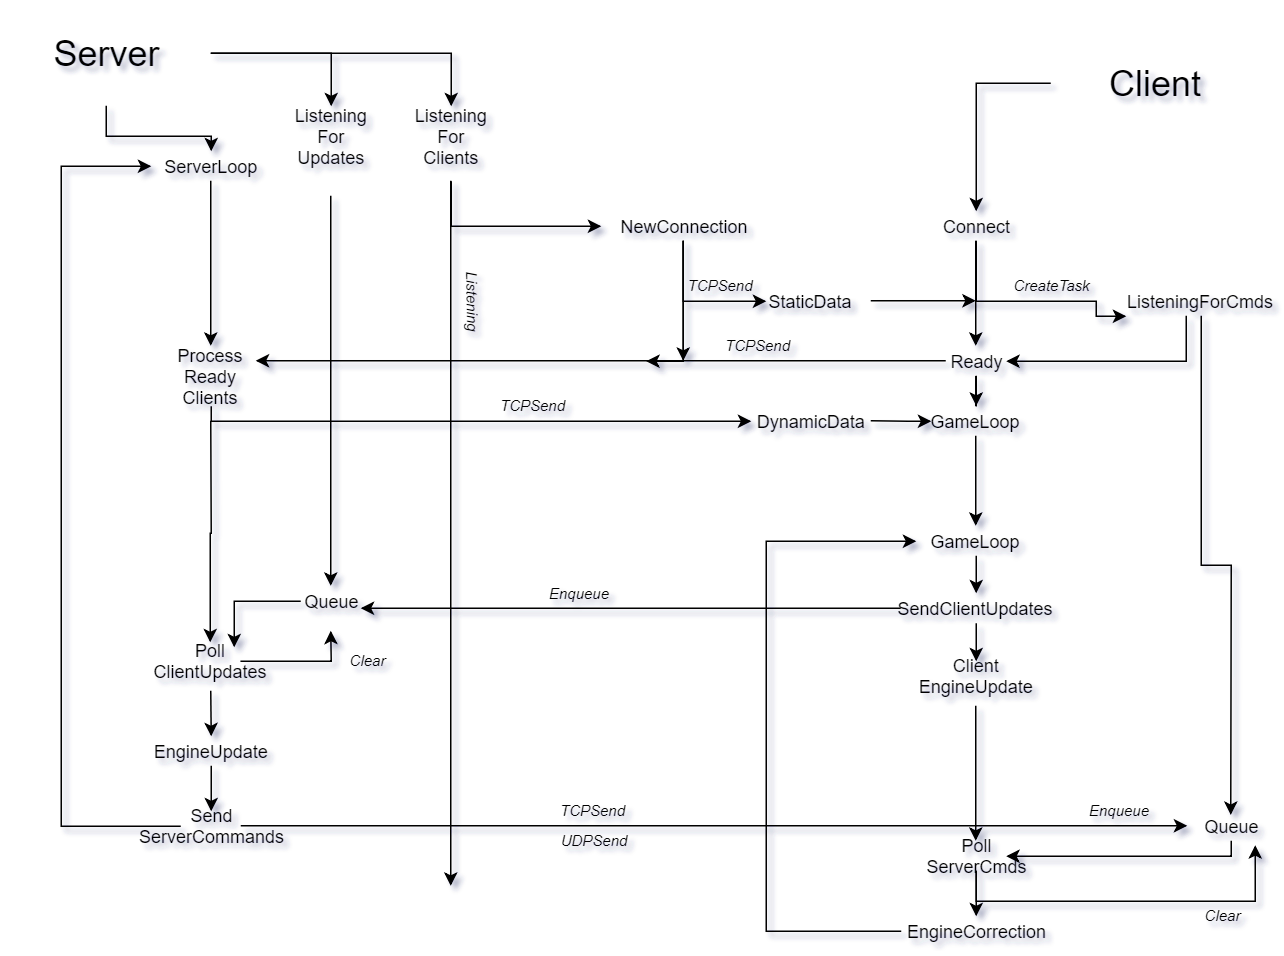
\includegraphics[width=\textwidth]{diagram.png}
\end{figure}

\end{document}
